\documentclass[conference]{IEEEtran}

\pdfoutput=1
\usepackage{enumitem}
\usepackage{hyperref}
\usepackage{tikz-cd}
\usepackage{url}
\usepackage{amsmath}
\usepackage{braket}
\usepackage{amsfonts}
\usepackage{amsthm}
\usepackage{amssymb}
\usepackage{graphicx}
\usepackage{caption}
\usepackage{subcaption}
\usepackage{float}
\usepackage{siunitx}
\usepackage{bbm}
\usepackage{comment}
\usepackage{mathrsfs}
\usepackage{qcircuit}
\usepackage{booktabs}
\usepackage{pifont}
\newcommand{\cmark}{\ding{51}}
\newcommand{\xmark}{\ding{55}}

\newcommand{\tr}[0]{\mathrm{tr}}
\newtheorem{conjecture}{Conjecture}
\newtheorem{theorem}{Theorem}
\newtheorem{problem}[theorem]{Problem}
\newtheorem{definition}[theorem]{Definition}
\newtheorem{lemma}[theorem]{Lemma}
\newtheorem{corollary}[theorem]{Corollary}
% \newtheorem{algorithm}[theorem]{Algorithm} % conflicts with IEEEtran
\newcommand{\lem}[1]{\hyperref[lem:#1]{Lemma~\ref*{lem:#1}}}

\begin{document}

\title{Quantum Adaptive Self-Attention for Quantum Transformer Models}

\author{
  \IEEEauthorblockN{Chi-Sheng Chen}
  \IEEEauthorblockA{Neuro Industry Research\\
    Neuro Industry, Inc.\\
    Boston, MA, USA}
  \and
  \IEEEauthorblockN{En-Jui Kuo}
  \IEEEauthorblockA{Department of Electrophysics\\
    National Yang Ming Chiao Tung University\\
    Hsinchu, Taiwan, R.O.C.}
}

\maketitle

\begin{abstract}
Integrating quantum computing into deep learning architectures is a promising but poorly understood endeavor: when does a quantum layer actually help, and how much quantum is enough?
We address both questions through Quantum Adaptive Self-Attention (QASA), a hybrid Transformer that replaces the value projection in a \emph{single} encoder layer with a parameterized quantum circuit (PQC), while keeping all other layers classical.
This \emph{minimal quantum integration} strategy uses only 36 trainable quantum parameters---fewer than any competing quantum model---yet achieves the best MSE on 4 of 9 synthetic benchmarks and a 6.0\% MAE reduction on the real-world ETTh1 dataset.
An ablation study reveals that quantum layer \emph{position} matters more than \emph{count}: adding more quantum layers degrades performance, while placing a single layer at the optimal position yields up to $3\times$ improvement.
Comparison with two recent quantum time-series baselines---QLSTM and QnnFormer---confirms that QASA matches or exceeds models with $2$--$4\times$ more quantum parameters, significantly outperforming QLSTM on the seasonal trend task ($p{=}0.009$, Cohen's $d{>}6$).
Crucially, the benefit is \emph{task-conditional}: QASA excels on chaotic, noisy, and trend-dominated signals, while classical Transformers remain superior for clean periodic waveforms---providing a practical taxonomy for when quantum enhancement is warranted.
These findings establish an \emph{architectural parsimony} principle for hybrid quantum-classical design: maximal quantum benefit is achieved not by maximizing quantum resources, but by strategically placing minimal quantum computation where it matters most.
\end{abstract}



\section{Introduction}
Transformer architectures~\cite{vaswani2017attention} have become the backbone of modern deep learning, powering state-of-the-art models across natural language processing, computer vision, and sequential prediction. Their core strength lies in the self-attention mechanism, which dynamically models long-range dependencies. However, this comes at a significant computational cost---quadratic in sequence length---motivating the search for alternative attention paradigms.

Quantum computing offers a compelling candidate: parameterized quantum circuits (PQCs) operate in exponentially large Hilbert spaces and can represent correlations that are classically intractable to express compactly~\cite{havlicek2019supervised}. Recent work has explored quantum-enhanced sequence models, including quantum LSTMs~\cite{chen2022quantum} and quantum Transformer variants~\cite{cai2024qnnformer}, which replace classical components wholesale with variational quantum circuits. However, a fundamental question remains unanswered: \emph{how much quantum integration is actually beneficial, and where should it be placed?}

In this work, we propose Quantum Adaptive Self-Attention (QASA), a hybrid architecture designed around a principle of \textbf{architectural parsimony}---the idea that maximal quantum benefit comes not from maximizing quantum resources, but from placing minimal quantum computation at the optimal position. QASA retains $N{-}1$ classical Transformer encoder layers and replaces only the value projection in the \emph{final} layer with a PQC, using just 36 trainable quantum parameters. This stands in contrast to approaches such as QLSTM (128 quantum parameters) and QnnFormer (90 quantum parameters), which distribute quantum computation across the entire model.

Our systematic evaluation across nine synthetic benchmarks, one real-world dataset, three quantum baselines, and a comprehensive ablation study yields three key findings:




\subsection{Contributions}
\begin{itemize}
    \item \textbf{Architectural parsimony principle.} We demonstrate that a single quantum-enhanced layer outperforms architectures with 2--4$\times$ more quantum parameters. Our ablation study shows that quantum layer \emph{position} matters more than \emph{count}: increasing quantum layers from one to four degrades performance on most tasks, while placing one layer at the optimal position yields up to $3\times$ improvement over the classical baseline.

    \item \textbf{Task-conditional quantum advantage taxonomy.} We provide empirical evidence that quantum enhancement benefits specific signal classes---chaotic dynamics, noisy oscillations, and smooth trends---while classical Transformers remain superior for clean periodic signals and sharp discontinuities. This taxonomy offers practitioners a principled guide for when to deploy hybrid quantum-classical models.

    \item \textbf{Comprehensive empirical validation.} QASA achieves the best MSE on 4 of 9 benchmarks (tied with the classical baseline), significantly outperforms QLSTM on the seasonal trend task ($p{=}0.009$), and reduces MAE by 6.0\% on the real-world ETTh1 dataset. These results hold across multiple random seeds and are supported by statistical significance tests, effect size analysis, and non-parametric Friedman tests.

\end{itemize}

\begin{figure}
    \centering
    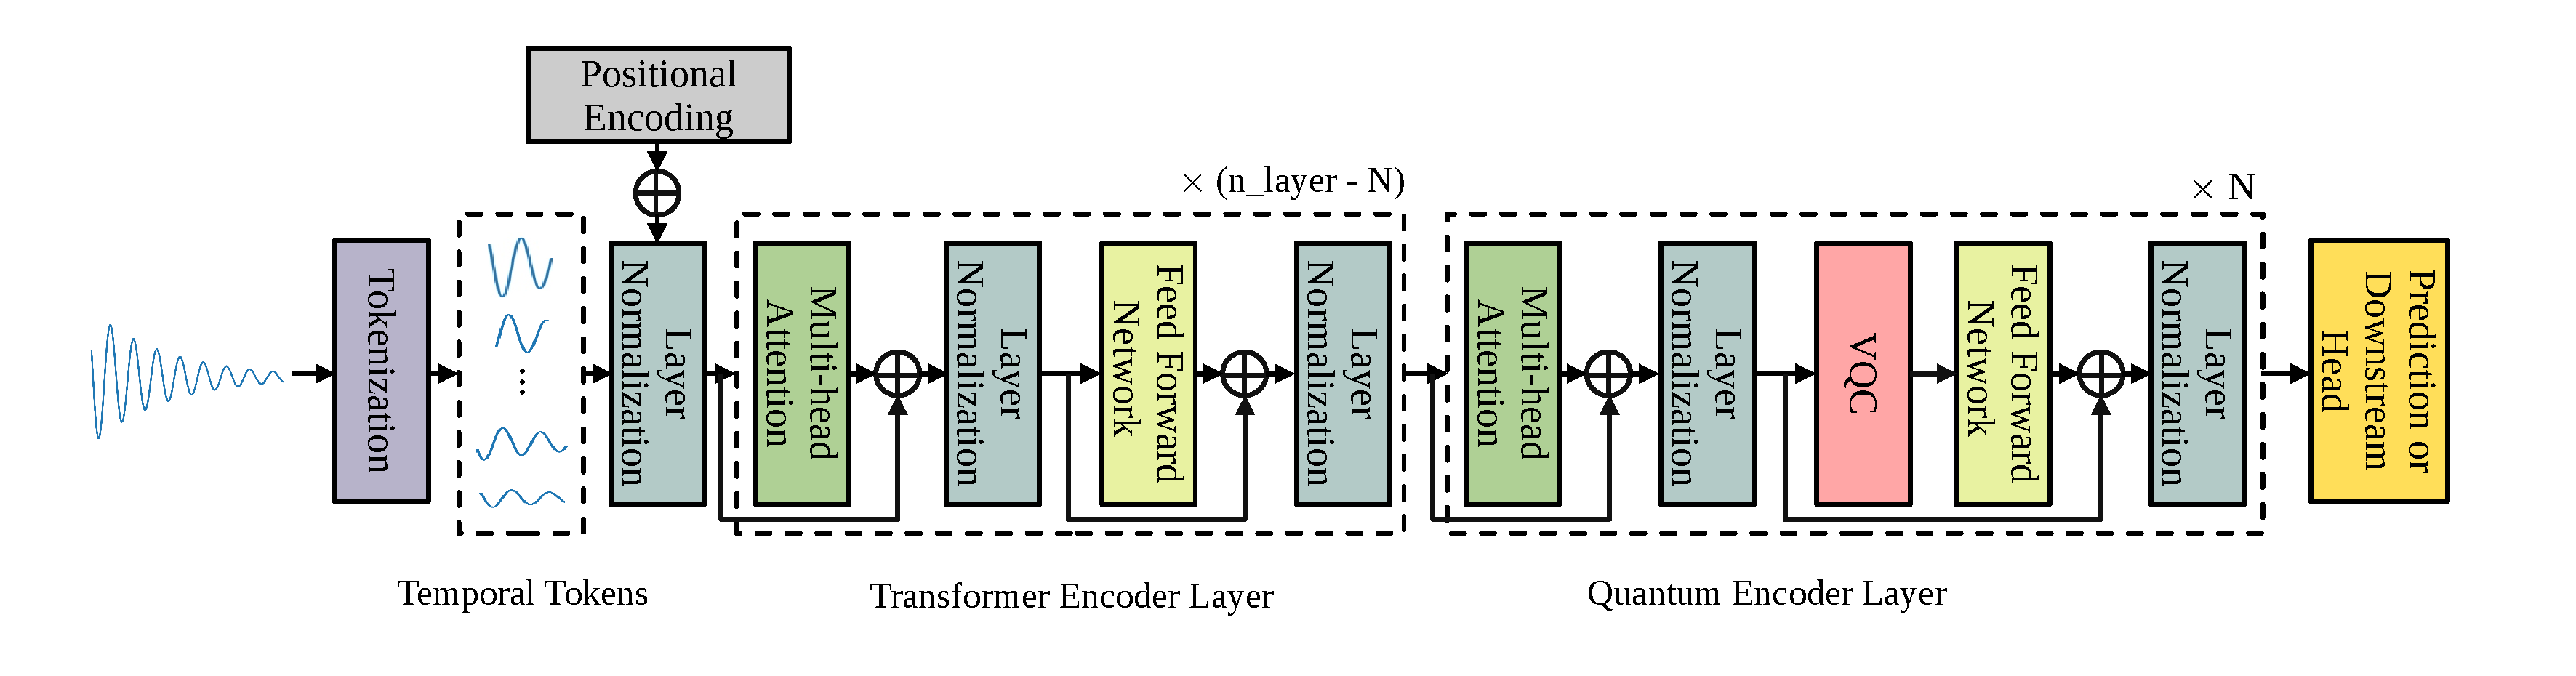
\includegraphics[width=1.1\linewidth]{img/QASA.pdf}
    \caption{Overview of the QASA architecture. The model consists of $N{-}1$ standard Transformer encoder layers followed by one Quantum Encoder Layer. The Quantum Encoder Layer replaces the value projection in self-attention with a parameterized quantum circuit (PQC) operating on 8 qubits with 4 variational layers, followed by a classical feedforward network with residual connections.}
    \label{fig:qasa}
\end{figure}


\section{Related work}
\subsection{Deep Learning on Time-Series Data}
Deep learning has significantly advanced the modeling and understanding of time-series data across various domains. Recurrent Neural Networks (RNNs) \cite{schuster1997bidirectional}, particularly Long Short-Term Memory (LSTM) networks \cite{hochreiter1997long} and Gated Recurrent Units (GRUs) \cite{chung2014empirical}, have been widely adopted due to their ability to capture long-term temporal dependencies. However, their sequential nature limits parallelization and increases training time. To address this, temporal convolutional networks (TCNs) \cite{lea2017temporal} and Transformer-based architectures \cite{vaswani2017attention} have demonstrated superior performance by enabling parallel processing and better long-range dependency modeling. 


In industrial and scientific applications, Transformer variants such as the Temporal Fusion Transformer (TFT) \cite{lim2021temporal} and Informer \cite{zhou2021informer} have been applied to multi-horizon prediction tasks with irregular time intervals and exogenous variables. Similar time-series learning techniques have been applied successfully in molecular dynamics and open quantum systems \cite{tsai2022path, tsai2020learning}.

Despite these advancements, challenges remain in modeling noisy, sparse, or irregularly-sampled sequences, motivating the development of hybrid models that integrate domain-specific priors with general-purpose deep learning architectures.

\subsection{Quantum Deep Learning on Time-Series Data}
While classical deep learning has achieved remarkable success in time-series analysis, it often requires extensive computational resources and large-scale data to generalize effectively. With the advent of quantum computing, Quantum Deep Learning (QDL) \cite{biamonte2017quantum} has emerged as a promising paradigm for modeling complex temporal patterns, offering theoretical advantages in expressivity and optimization through quantum entanglement and superposition.

In the context of time-series data, several quantum-inspired architectures have been proposed. Variational Quantum Circuits (VQCs) \cite{gohel2024quantum} and Quantum Recurrent Neural Networks (QRNNs) \cite{takaki2021learning} have been introduced to capture temporal dependencies using parameterized quantum gates and recurrent structures. A particularly notable development is the Quantum Long Short-Term Memory (QLSTM) network \cite{chen2022quantum}, which integrates quantum circuits into the gating mechanisms of classical LSTMs. Recent comprehensive benchmarking studies \cite{fellner2025quantum_benchmark} have compared VQC-based regression against classical GRU and LSTM models, finding that while classical models often lead in raw accuracy, VQCs exhibit higher robustness to noise and better generalization on small-scale datasets.

Recent work has further expanded quantum approaches for temporal data. Tang et al.~\cite{tang2026qnnformer} proposed Qnnformer, a multi-attention mechanism leveraging quantum circuits for long-term forecasting, achieving significant error reductions on benchmark datasets. Chakraborty and Heintz~\cite{chakraborty2025qcaapatch} integrated hybrid quantum-classical attention into patch-based transformers for multivariate forecasting. Chittoor et al.~\cite{chittoor2024qultsf} developed QuLTSF for long-term forecasting with quantum neural networks, demonstrating advantages in convergence stability for non-stationary data. Laskar and Goel~\cite{laskar2025shallow} investigated the impact of different entanglement topologies in shallow circuits for time-series prediction on NISQ hardware. In finance, quantum-enhanced architectures have been investigated for demand prediction and volatility modeling \cite{paquet2022quantumleap}.

Despite these advancements, research on Quantum Transformers for time-series data remains limited. Most existing studies focus on Quantum Visual Transformers (QViT) \cite{cherrat2022quantum} or fully quantum architectures such as Quixer \cite{khatri2024quixer} in sequence modeling, leaving a gap in understanding how hybrid quantum-classical self-attention mechanisms can be practically deployed for temporal forecasting. Addressing this gap is the key focus of this work.


\section{Methodology}
\begin{figure*}
    \centering
    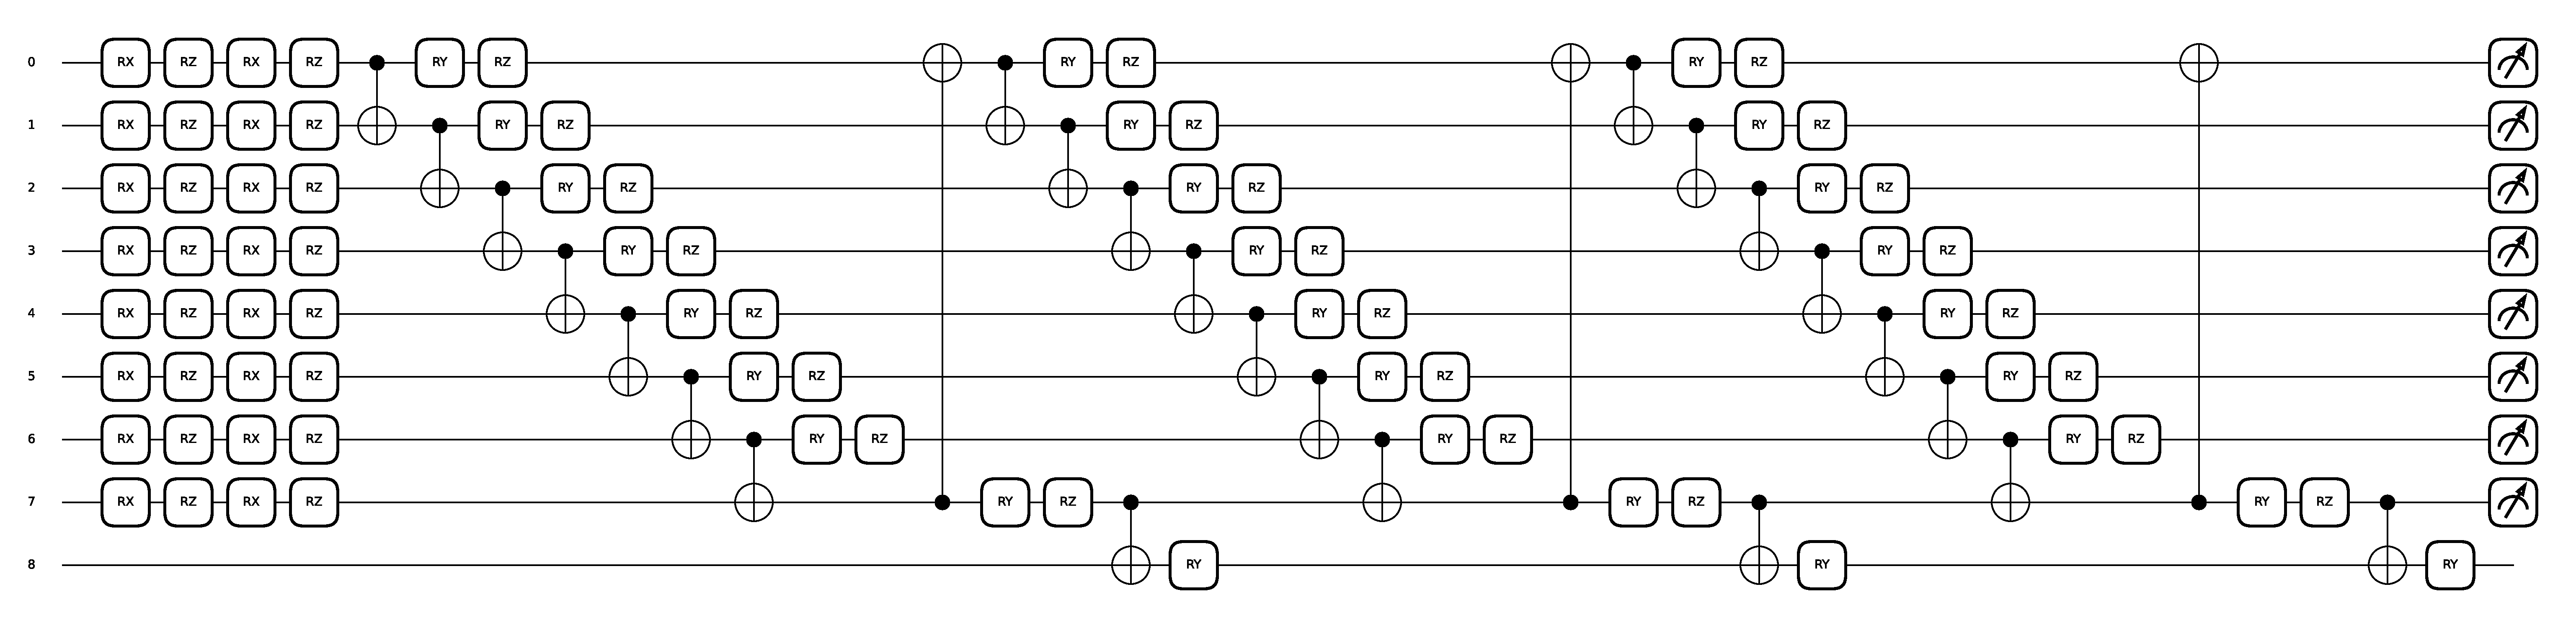
\includegraphics[width=1\linewidth]{img/quantum_circuit_diagram.pdf}
    \caption{The parameterized quantum circuit (PQC) used in QASA's QuantumLayer. The circuit operates on $n{=}8$ data qubits plus one ancilla qubit, with $L{=}4$ variational layers. Each layer applies single-qubit rotations ($R_X$, $R_Y$, $R_Z$) and CNOT entangling gates in a ring topology. Input features are encoded via $R_X$ and $R_Z$ rotations on each qubit, and the output is obtained by measuring $\langle Z_i \rangle$ on all data qubits.}
    \label{fig:qasa_qnn}
\end{figure*}



\begin{table}[h]
\centering
\caption{Quantum Adaptive Self-Attention (QASA) Transformer Architecture. Each row lists a layer with its operation and input/output tensor shapes.
$L$ denotes the input sequence length (e.g., $L{=}50$), 
$d$ is the hidden feature dimension (e.g., $d{=}256$), 
and $n$ is the number of qubits in the quantum circuit (e.g., $n{=}8$). ‘Attn’ is an abbreviation for ‘attention’.}
\label{tab:model-architecture}
\begin{tabular}{l l c c }
\hline
\textbf{Layer} & \textbf{Operation} & \textbf{Input Shape} & \textbf{Output Shape} \\
\hline
Input & Raw sequence & $(L, 1)$ & $(L, 1)$ \\
% \hline
Linear Embedding & Linear + LayerNorm & $(L, 1)$ & $(L, d)$ \\
% \hline
Positional Encoding & Add sinusoidal PE & $(L, d)$ & $(L, d)$ \\
% \hline
Transformer Layer $\times (N{-}1)$ & Multihead Attn + FFN & $(L, d)$ & $(L, d)$ \\
% \hline
Quantum Encoder Layer & \begin{tabular}[c]{@{}l@{}}Self-Attn + QNN + FFN\end{tabular} & $(L, d)$ & $(L, d)$ \\
% \hline
\quad QuantumLayer (QNN) & \begin{tabular}[c]{@{}l@{}}Linear $\rightarrow \mathbb{R}^n$ \\ PQC $\rightarrow \mathbb{R}^n$ \\ Linear $\rightarrow \mathbb{R}^d$ + Residual\end{tabular} & $(L, d)$ & $(L, d)$ \\
% \hline
Final Linear & Extract $h[L]$ and project & $(d)$ & $(1)$ \\
\hline
\end{tabular}
\end{table}



\subsection{Overview}

We propose a hybrid quantum-classical Transformer model tailored for sequential data forecasting. The architecture is designed to capture temporal dependencies through classical attention mechanisms, while integrating a parameterized quantum circuit (PQC) to enhance the model's expressiveness and representation power.

Given an input sequence $x \in \mathbb{R}^{L \times 1}$ of length $L$, our model predicts a scalar target $\hat{y} \in \mathbb{R}$ corresponding to the next value in the sequence.

\subsection{Embedding and Positional Encoding}

The input sequence is first projected into a high-dimensional space using a linear layer, followed by layer normalization:
\begin{equation}
h_0 = \text{LayerNorm}(W_e x + b_e), \quad h_0 \in \mathbb{R}^{L \times d},
\end{equation}
where $d$ is the hidden dimension. We then apply fixed sinusoidal positional encoding to inject temporal order information:
\begin{equation}
h_0 \leftarrow h_0 + PE,
\end{equation}
where $PE$ denotes the positional encoding matrix.

\subsection{Transformer Encoder Layers}

The encoder consists of $N$ layers, where the first $N-1$ layers are standard Transformer encoder layers defined as:
\begin{equation}
h_i = \text{Transformer}(h_{i-1}), \quad i = 1, \dots, N-1.
\end{equation}

The Transformer layer consists of two main sublayers: a multi-head self-attention mechanism and a position-wise feed-forward network (FFN). Each sublayer is wrapped with a residual connection and layer normalization. Formally, the computation of the $i$-th Transformer layer can be described as follows:
\begin{align}
z_i &= \text{LayerNorm}\left(h_{i-1} + \text{MultiHeadSelfAttention}(h_{i-1})\right), \\
h_i &= \text{LayerNorm}\left(z_i + \text{FFN}(z_i)\right).
\end{align}

The multi-head self-attention mechanism is defined as:
\begin{equation}
\text{MultiHeadSelfAttention}(X) = \text{Concat}(head_1, \dots, head_H)W^O,
\end{equation}
where each attention head is computed as:
\begin{equation}
head_j = \text{Attention}(XW_j^Q, XW_j^K, XW_j^V), \quad j = 1, \dots, H.
\end{equation}

In the self-attention mechanism, each input vector is linearly projected into three different spaces to form the \textbf{query} ($Q$), \textbf{key} ($K$), and \textbf{value} ($V$) matrices:
\begin{equation}\label{eq:at}
Q = XW^Q, \quad K = XW^K, \quad V = XW^V,
\end{equation}
where $X \in \mathbb{R}^{T \times d_{\text{model}}}$ is the input sequence (with $T$ tokens), and $W^Q, W^K, W^V \in \mathbb{R}^{d_{\text{model}} \times d_k}$ are learnable projection matrices.

The roles of $Q$, $K$, and $V$ are as follows:
\begin{itemize}
  \item \textbf{Query ($Q$)}: Represents the current token's request for information.
  \item \textbf{Key ($K$)}: Represents the "content" or identity of each token in the sequence.
  \item \textbf{Value ($V$)}: Represents the actual information to be retrieved.
\end{itemize}

The attention mechanism computes a similarity score between each query and all keys:
\begin{equation}
\text{Attention}(Q, K, V) = \text{softmax}\left( \frac{QK^\top}{\sqrt{d_k}} \right) V.
\end{equation}
This allows the model to retrieve contextually relevant information by weighting each value according to the query-key similarity.


The feed-forward network (FFN) is applied to each position separately and identically:
\begin{equation}
\text{FFN}(x) = \max(0, xW_1 + b_1)W_2 + b_2,
\end{equation}
where $W_1, W_2, b_1, b_2$ are learnable parameters.

Thus, the Transformer block can be summarized as:
\begin{equation}
z_i = \mathrm{LayerNorm}\big(h_{i-1} + \mathrm{MultiHeadSelfAttention}(h_{i-1})\big), 
\end{equation}
\begin{equation}
h_i = \mathrm{LayerNorm}\big(z_i + \mathrm{FFN}(z_i)\big), 
\end{equation}
\begin{equation}
\text{Transformer}(h_{i-1}) = h_i.
\end{equation}




Each Transformer encoder layer includes multi-head self-attention, residual connections, and feedforward networks with GELU activation.

\subsection{Quantum Encoder Layer}

The final encoder block is a quantum-enhanced encoder layer. It begins with a multi-head self-attention module:
\begin{equation}
a = \text{MultiHeadAttention}(h_{N-1}) = \text{Concat}(head_1, \ldots, head_h)W^O,
\end{equation}
\begin{equation}
\text{where } head_i = \text{Attention}(QW_i^Q, KW_i^K, VW_i^V),
\end{equation}
\begin{equation}
\text{Attention}(Q, K, V) = \text{softmax}\left(\frac{QK^T}{\sqrt{d_k}}\right)V,
\end{equation}

\begin{equation}
h' = \text{LayerNorm}(h_{N-1} + a).
\end{equation}



Each token vector $h'_i \in \mathbb{R}^d$ is passed through a quantum layer. The quantum layer first linearly projects the input to a lower-dimensional space suitable for quantum encoding:
\begin{equation}
h_q = \tanh(W_q h'_i),
\end{equation}
where $h_q \in \mathbb{R}^{n}$ and $n$ is the number of qubits.

The vector $h_q$ is then passed as input to a parameterized quantum circuit (PQC), which is defined over $n + 1$ qubits and $L_q$ layers of unitary operations. The PQC applies data re-uploading using $RX$ and $RZ$ gates, and introduces entanglement using $CNOT$ and $RY$ gates. The final output is computed as the expectation values of Pauli-Z operators on the first $n$ qubits:
\begin{equation}
\text{QC}(h_q) = \left[ \langle Z_j \rangle \right]_{j=1}^{n}.
\end{equation}

The quantum output is then projected back to the original dimension and added residually:
\begin{equation}
z_i = h'_i + W_o \cdot \text{QC}(h_q + t),
\end{equation}
where $t$ denotes the timestep (i.e., sequence length), added as a conditioning signal.

Finally, a feedforward network with GELU activation is applied, followed by layer normalization:
\begin{equation}
h_N = \text{LayerNorm}(z + \text{FFN}(z)).
\end{equation}

\paragraph{QuantumLayer: Residual Quantum Projection with Conditional Reuploading.}

To enrich the representational capacity of the Transformer encoder, we introduce a novel \texttt{QuantumLayer} module that integrates parameterized quantum circuits (PQC) into a residual learning structure. Each token embedding $x \in \mathbb{R}^d$ is first projected into a quantum-compatible latent space $\mathbb{R}^n$, where $n$ denotes the number of qubits:

\begin{equation}
h_q = \tanh(W_q x) + t,
\end{equation}

where $W_q \in \mathbb{R}^{n \times d}$ is a learnable projection matrix, and $t$ is a scalar encoding of the sequence length, used to condition the quantum processing on global temporal context.

The resulting vector $h_q$ is fed into a parameterized quantum circuit $\text{QC}(\cdot)$ with $L_q$ layers and $n+1$ qubits, implemented using a data reuploading strategy. Each layer of the PQC applies a combination of single-qubit rotations ($RX$, $RZ$, $RY$) and entangling gates (e.g., $CNOT$), allowing the circuit to perform complex non-classical transformations:

\begin{equation}
\text{QC}(h_q) = \left[ \langle Z_j \rangle \right]_{j=1}^{n},
\end{equation}

where $\langle Z_j \rangle$ denotes the expectation value of the Pauli-$Z$ operator measured on qubit $j$.

The output from the quantum circuit is then projected back to the original feature space and added to the input as a residual enhancement:

\begin{equation}
\text{QuantumLayer}(x, t) = x + W_o \cdot \text{QC}(h_q),
\end{equation}

where $W_o \in \mathbb{R}^{d \times n}$ is a learnable linear projection. This design allows the model to leverage the expressive power of quantum circuits within a fully differentiable classical framework. The quantum circuit acts as a learnable nonlinear operator conditioned on both the feature vector and temporal context, enabling richer transformations than classical feedforward layers of similar capacity.

\paragraph{Hybrid Classical-Quantum Encoding.}

In our design, we adopt a hybrid encoder composed of $(N{-}1)$ standard Transformer encoder layers followed by a single quantum-enhanced encoder layer. This layered configuration offers a practical and effective trade-off between scalability and expressiveness. Specifically, the classical Transformer blocks serve as powerful hierarchical feature extractors with stable training dynamics, while the quantum encoder layer provides a complementary inductive bias via entangled quantum operations and high-dimensional projection.

By placing the quantum block at the final stage of the encoder, the model benefits from:
\begin{itemize}
    \item \textbf{Stable gradient propagation:} Classical layers handle early-stage representation learning, mitigating the vanishing gradient problem that may arise in purely quantum-based models.
    \item \textbf{Enhanced non-classical feature transformation:} The quantum circuit introduces expressive transformations that cannot be easily replicated by shallow classical networks, enabling the model to capture global correlations and nonlinearities more efficiently.
    \item \textbf{Efficient resource usage:} Since only a single quantum layer is used, the model maintains compatibility with current noisy intermediate-scale quantum (NISQ) hardware, and avoids the overhead of full quantum depth throughout the network.
\end{itemize}

This hybrid composition allows the model to leverage the strengths of both classical and quantum computation in a synergistic manner, enabling end-to-end training on standard hardware with enhanced representation capability for sequential learning tasks.

\begin{figure*}[htbp]
  \centering
  
  % Row 1: Model A
  \begin{subfigure}[b]{0.3\textwidth}
    
\includegraphics[width=\textwidth]{img/single_transformer/epoch_1.png}
    \caption{Traditional Transformer - Epoch 1}
  \end{subfigure}
  \begin{subfigure}[b]{0.3\textwidth}
    
\includegraphics[width=\textwidth]{img/single_transformer/epoch_15.png}
    \caption{Traditional Transformer - Epoch 15}
  \end{subfigure}
  \begin{subfigure}[b]{0.3\textwidth}
    
\includegraphics[width=\textwidth]{img/single_transformer/epoch_30.png}
    \caption{Traditional Transformer - Epoch 30}
  \end{subfigure}
  
  % Row 2: Model B
  \begin{subfigure}[b]{0.3\textwidth}
    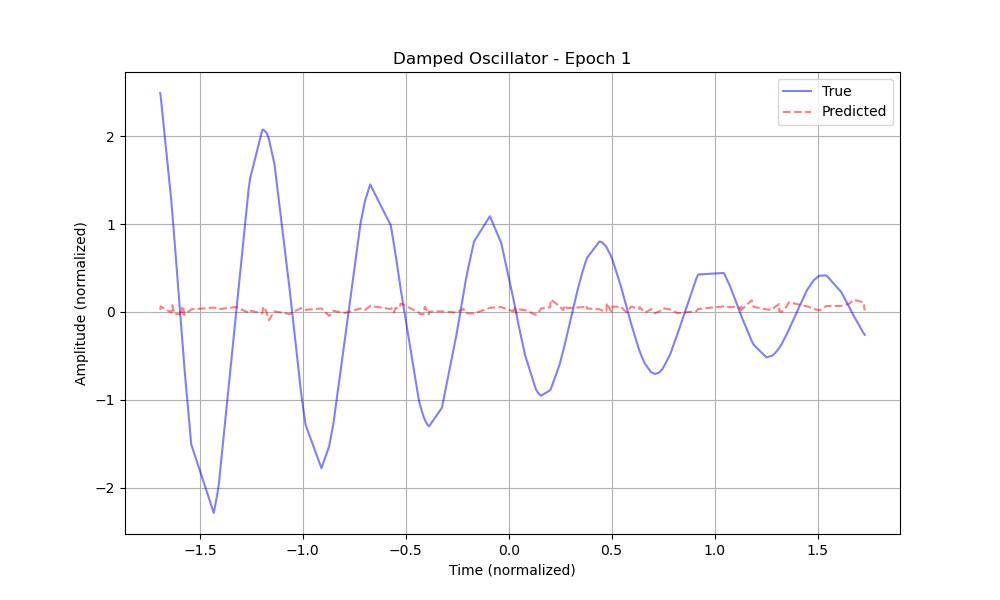
\includegraphics[width=\textwidth]{img/c_qasa/epoch_1.png}
    \caption{$QASA_{classical}$ - Epoch 1}
  \end{subfigure}
  \begin{subfigure}[b]{0.3\textwidth}
    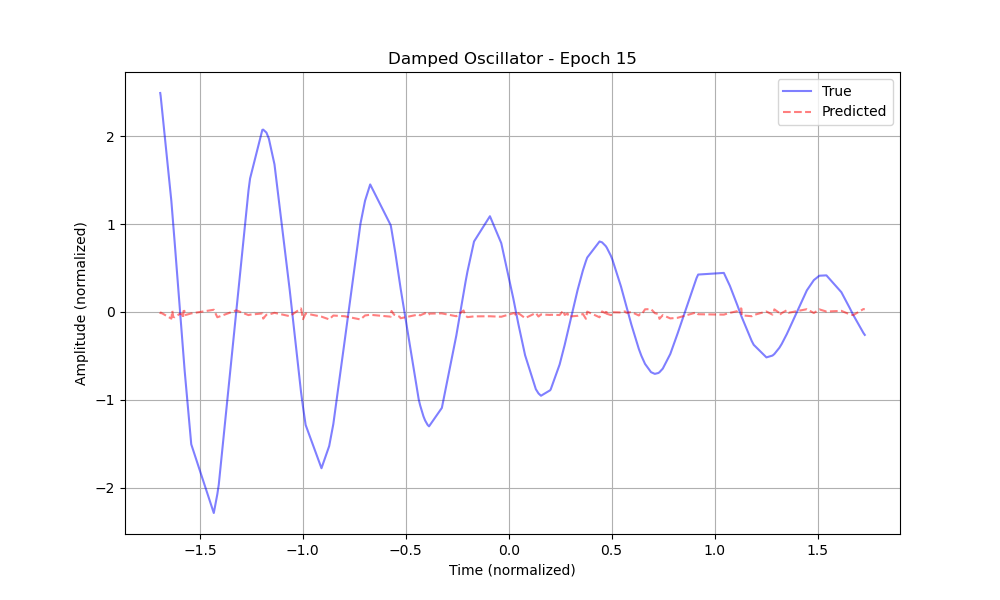
\includegraphics[width=\textwidth]{img/c_qasa/epoch_15.png}
    \caption{$QASA_{classical}$ - Epoch 15}
  \end{subfigure}
  \begin{subfigure}[b]{0.3\textwidth}
    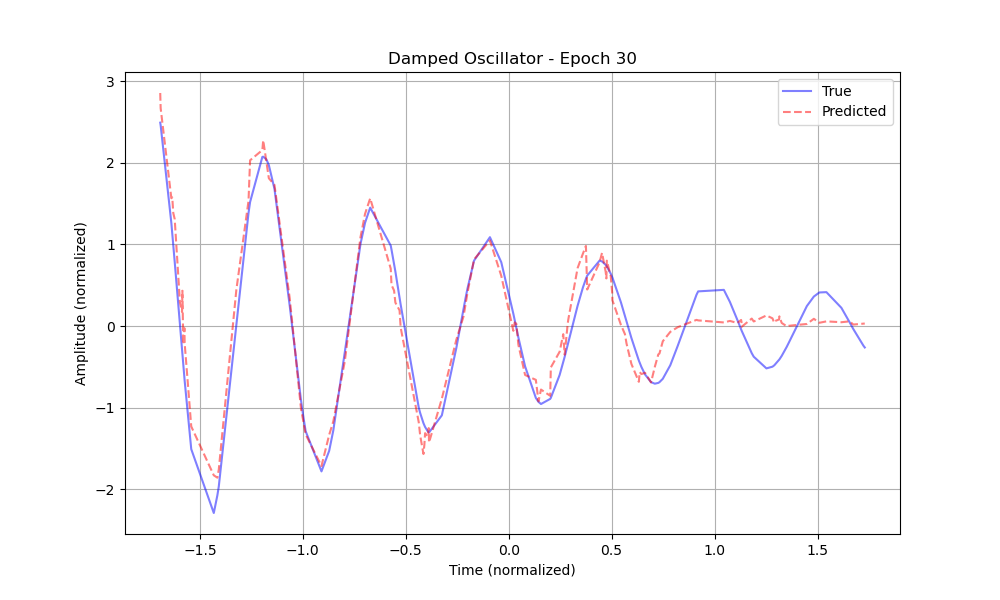
\includegraphics[width=\textwidth]{img/c_qasa/epoch_30.png}
    \caption{$QASA_{classical}$ - Epoch 30}
  \end{subfigure}
  
  % Row 3: Model C
  \begin{subfigure}[b]{0.3\textwidth}
    
\includegraphics[width=\textwidth]{img/q_qasa/epoch_1.png}
    \caption{$QASA$ - Epoch 1}
  \end{subfigure}
  \begin{subfigure}[b]{0.3\textwidth}
    
\includegraphics[width=\textwidth]{img/q_qasa/epoch_15.png}
    \caption{$QASA$ - Epoch 15}
  \end{subfigure}
  \begin{subfigure}[b]{0.3\textwidth}
    
\includegraphics[width=\textwidth]{img/q_qasa/epoch_30.png}
    \caption{$QASA$ - Epoch 30}
  \end{subfigure}
  
  \caption{
Visual comparison of prediction performance across three models—Traditional Transformer, \( \text{QASA}_{\text{classical}} \), and QASA—at epochs 1, 15, and 30 on the damped oscillator task. At epoch 1, all models show poor predictions. By epoch 15, QASA already demonstrates significantly improved alignment with the true signal, while the other models lag behind. At epoch 30, QASA achieves near-perfect predictions, indicating much faster convergence compared to both the classical and transformer baselines.
}
\end{figure*}

\paragraph{Gate Composition in QuantumLayer.}

The design of the parameterized quantum circuit (PQC) in the \texttt{QuantumLayer} follows a data reuploading and entanglement-aware structure optimized for hybrid neural architectures. Each layer of the PQC is composed of three primary stages:

\begin{enumerate}
    \item \textbf{Data Encoding via Single-Qubit Rotations:} The input features are encoded into quantum states using $RX$ and $RZ$ gates per qubit:
    \begin{equation}
    \forall i \in \{0, \dots, n-1\}, \quad \text{Apply } RX(x_i),\ RZ(x_i) \text{ on wire } i.
    \end{equation}

    This approach ensures both amplitude and phase information from classical features are embedded into the quantum state.

    \item \textbf{Parameterized Rotations with Data Reuploading:} Across $L_q$ layers, the circuit includes learnable $RY$ and $RZ$ rotations:
    \begin{equation}
    RY(\theta_{l, i})\ RZ(\theta_{l, i}) \quad \forall i, \forall l \in \{1, \dots, L_q\},
    \end{equation}
    enabling expressive nonlinear transformations and allowing the model to approximate highly non-classical mappings through repeated encoding.

    \item \textbf{Entanglement via Circular \texttt{CNOT} Topology:} To capture feature interactions across qubits, entanglement is introduced via a ring of $CNOT$ gates:
    \begin{equation}
    \text{CNOT}(i \rightarrow (i+1) \mod n),\quad \text{for } i = 0 \dots n{-}1.
    \end{equation}

    An additional CNOT is applied from the final qubit to an auxiliary $(n+1)$-th qubit, allowing enhanced control or global interaction effects:
    \begin{equation}
    \text{CNOT}(n{-}1 \rightarrow n),\quad RY(\theta_{l, n}) \text{ on wire } n.
    \end{equation}
\end{enumerate}

This gate configuration balances expressiveness and hardware feasibility. The use of simple universal gates ($RX, RZ, RY$, CNOT) ensures compatibility with most current quantum hardware, while circular entanglement introduces full connectivity with only $n$ CNOTs per layer, avoiding unnecessary depth. The auxiliary $(n+1)$-th qubit also serves as a tunable global channel, useful for capturing long-range dependencies in the encoded features.

\subsection{Circuit Expressibility and Entanglement Analysis}

To characterize the representational capacity of the QASA quantum circuit beyond its architectural description, we evaluate three established metrics from the quantum circuit benchmarking literature: entanglement entropy, the Meyer--Wallach entangling capability measure, and expressibility.

\paragraph{Entanglement Entropy.}
We compute the bipartite von Neumann entropy $S(\rho_A) = -\tr(\rho_A \log_2 \rho_A)$ across a balanced bipartition of the data qubits (qubits 0--3 vs.\ 4--7 plus auxiliary), averaged over 200 random parameter samples. The QASA circuit achieves a mean entanglement entropy of $2.26 \pm 0.12$ bits out of a maximum of 4.0 bits (normalized: 0.57), indicating substantial but not maximal entanglement. This moderate level is desirable: it ensures non-trivial quantum correlations across qubit subsets without collapsing into a maximally entangled state that would limit trainability~\cite{mcclean2018barren}.

\paragraph{Meyer--Wallach Entangling Capability.}
The Meyer--Wallach measure $Q(|\psi\rangle) \in [0, 1]$ quantifies the global entanglement of a pure state, with $Q = 0$ for product states and $Q = 1$ for maximally entangled states~\cite{meyer2002global}. Averaged over 1{,}000 random parameterizations, QASA achieves $Q = 0.981$, substantially higher than QLSTM ($Q = 0.710$) and QnnFormer ($Q = 0.883$). This confirms that the ring-topology CNOT structure with auxiliary qubit coupling generates near-maximally entangled states, despite using fewer two-qubit gates than QLSTM (27 vs.\ 56 CNOTs).

\paragraph{Expressibility.}
Following Sim et al.~\cite{sim2019expressibility}, we estimate expressibility by comparing the distribution of state fidelities $|\langle \psi(\theta_1) | \psi(\theta_2) \rangle|^2$ (for 5{,}000 random parameter pairs) against the Haar-random distribution via the Kullback--Leibler divergence. QASA yields $D_{\mathrm{KL}} = 0.029$, comparable to QnnFormer ($D_{\mathrm{KL}} = 0.026$) and substantially better than QLSTM ($D_{\mathrm{KL}} = 0.125$). Lower $D_{\mathrm{KL}}$ indicates wider coverage of the Hilbert space, a necessary condition for effective variational learning.

\begin{table}[h]
\centering
\caption{Comparative quantum circuit analysis across all three quantum models (5{,}000 parameter samples for expressibility, 1{,}000 for entangling capability). Lower expressibility KL divergence indicates wider Hilbert space coverage; higher Meyer--Wallach $Q$ indicates stronger entanglement generation.}
\label{tab:circuit_analysis}
\resizebox{\columnwidth}{!}{
\begin{tabular}{lcccccc}
\toprule
\textbf{Circuit} & \textbf{Qubits} & \textbf{Q-Params} & \textbf{CNOT Gates} & \textbf{Total Gates} & \textbf{Expr.\ ($D_{\mathrm{KL}}\downarrow$)} & \textbf{Ent.\ Cap.\ ($Q\uparrow$)} \\
\midrule
QASA & 9 & 36 & 27 & 110 & 0.029 & \textbf{0.981} \\
QLSTM & 8 & 32 & 56 & 104 & 0.125 & 0.710 \\
QnnFormer & 8 & 24 & 21 & 94 & \textbf{0.026} & 0.883 \\
\bottomrule
\end{tabular}
}
\end{table}

Table~\ref{tab:circuit_analysis} reveals a striking efficiency gap: QASA achieves the highest entangling capability ($Q = 0.981$) with only 27 CNOT gates, while QLSTM requires more than twice as many CNOTs (56) yet produces the weakest entanglement ($Q = 0.710$). This demonstrates that QASA's ring topology---where each qubit is entangled with its neighbor in a circular arrangement---is fundamentally more efficient than QLSTM's linear chain topology. QnnFormer achieves competitive expressibility with the fewest total gates (94), but its entangling power remains below QASA's. These results provide a circuit-level explanation for QASA's strong empirical performance: near-maximal entanglement enables the quantum layer to capture complex correlations, while high expressibility ensures the circuit can represent diverse functions during training.


\subsection{Prediction and Training Objective}

The prediction is generated by extracting the final time step representation $h_N[L] \in \mathbb{R}^d$ and applying a linear projection:
\begin{equation}
\hat{y} = W_{out} \cdot h_N[L] + b_{out}.
\end{equation}

The model is trained using the Mean Squared Error (MSE) loss:
\begin{equation}
\mathcal{L}_{\text{MSE}} = \frac{1}{N} \sum_{i=1}^N (y_i - \hat{y}_i)^2.
\end{equation}

Optimization is performed with AdamW and a cosine annealing learning rate scheduler. We apply early stopping and save the model with the best validation loss. During training, we also visualize sorted and unsorted predictions to monitor performance.






\section{Results and Discussions}

% \begin{table*}[h]
% \centering
% \caption{Comparison of model architectures: Vanilla Transformer, $QASA_{classical}$, and $QASA$.}
% \begin{tabular}{ l c c c }
% \hline
% \textbf{Component} & \textbf{Transformer} & \textbf{$QASA_{classical}$} & \textbf{$QASA$ (Quantum-Augmented)} \\
% \hline
% Input Projection & Linear($1 \rightarrow 256$) & Linear($1 \rightarrow 256$) & Linear($1 \rightarrow 256$) + LayerNorm \\
% Positional Encoding & Sinusoidal & Sinusoidal & Sinusoidal \\
% Encoder Layers & 4$\times$ Transformer (8 heads) & 4$\times$ Transformer (4 heads) & 3$\times$ Transformer + 1$\times$ QuantumEncoderLayer \\
% Feedforward Dim & 1024 & 1024 & 1024 (post-quantum FFN) \\
% Activation Function & ReLU & GELU & GELU \\
% Quantum Component & \xmark & \xmark & \cmark\ 8-qubit, 4-layer VQC \\
% Output Layer & 2-layer MLP  (ReLU + Linear) & 2-layer MLP (GELU + Linear) & Linear(256 $\rightarrow$ 1) \\
% Attention Heads & 8 & 4 & 4 \\
% Hidden Dim & 256 & 256 & 256 \\
% \hline
% \end{tabular}
% \end{table*}
\begin{table}[h]
\centering
\caption{Comparison of model architectures: $QASA_{classical}$ and $QASA$.}
\label{tab:qasa-compare}
\resizebox{\textwidth}{!}{
\begin{tabular}{ l c c }
\hline
\textbf{Component} & \textbf{$QASA_{classical}$} & \textbf{$QASA$} \\
\hline
Input Projection & Linear($1 \rightarrow 256$) & Linear($1 \rightarrow 256$) + LayerNorm \\
Positional Encoding & Sinusoidal & Sinusoidal \\
Encoder Layers & 4$\times$ Transformer (4 heads) & 3$\times$ Transformer + 1$\times$ QuantumEncoderLayer \\
Feedforward Dim & 1024 & 1024 (post-quantum FFN) \\
Activation Function & GELU & GELU \\
Quantum Component & \xmark & \cmark\ 8-qubit, 4-layer VQC \\
Output Layer & 2-layer MLP (GELU + Linear) & Linear(256 $\rightarrow$ 1) \\
Attention Heads & 4 & 4 \\
Hidden Dim & 256 & 256 \\
\hline
\end{tabular}
}
\end{table}


\subsection{Experiment Details}
\begin{figure}
    \centering
    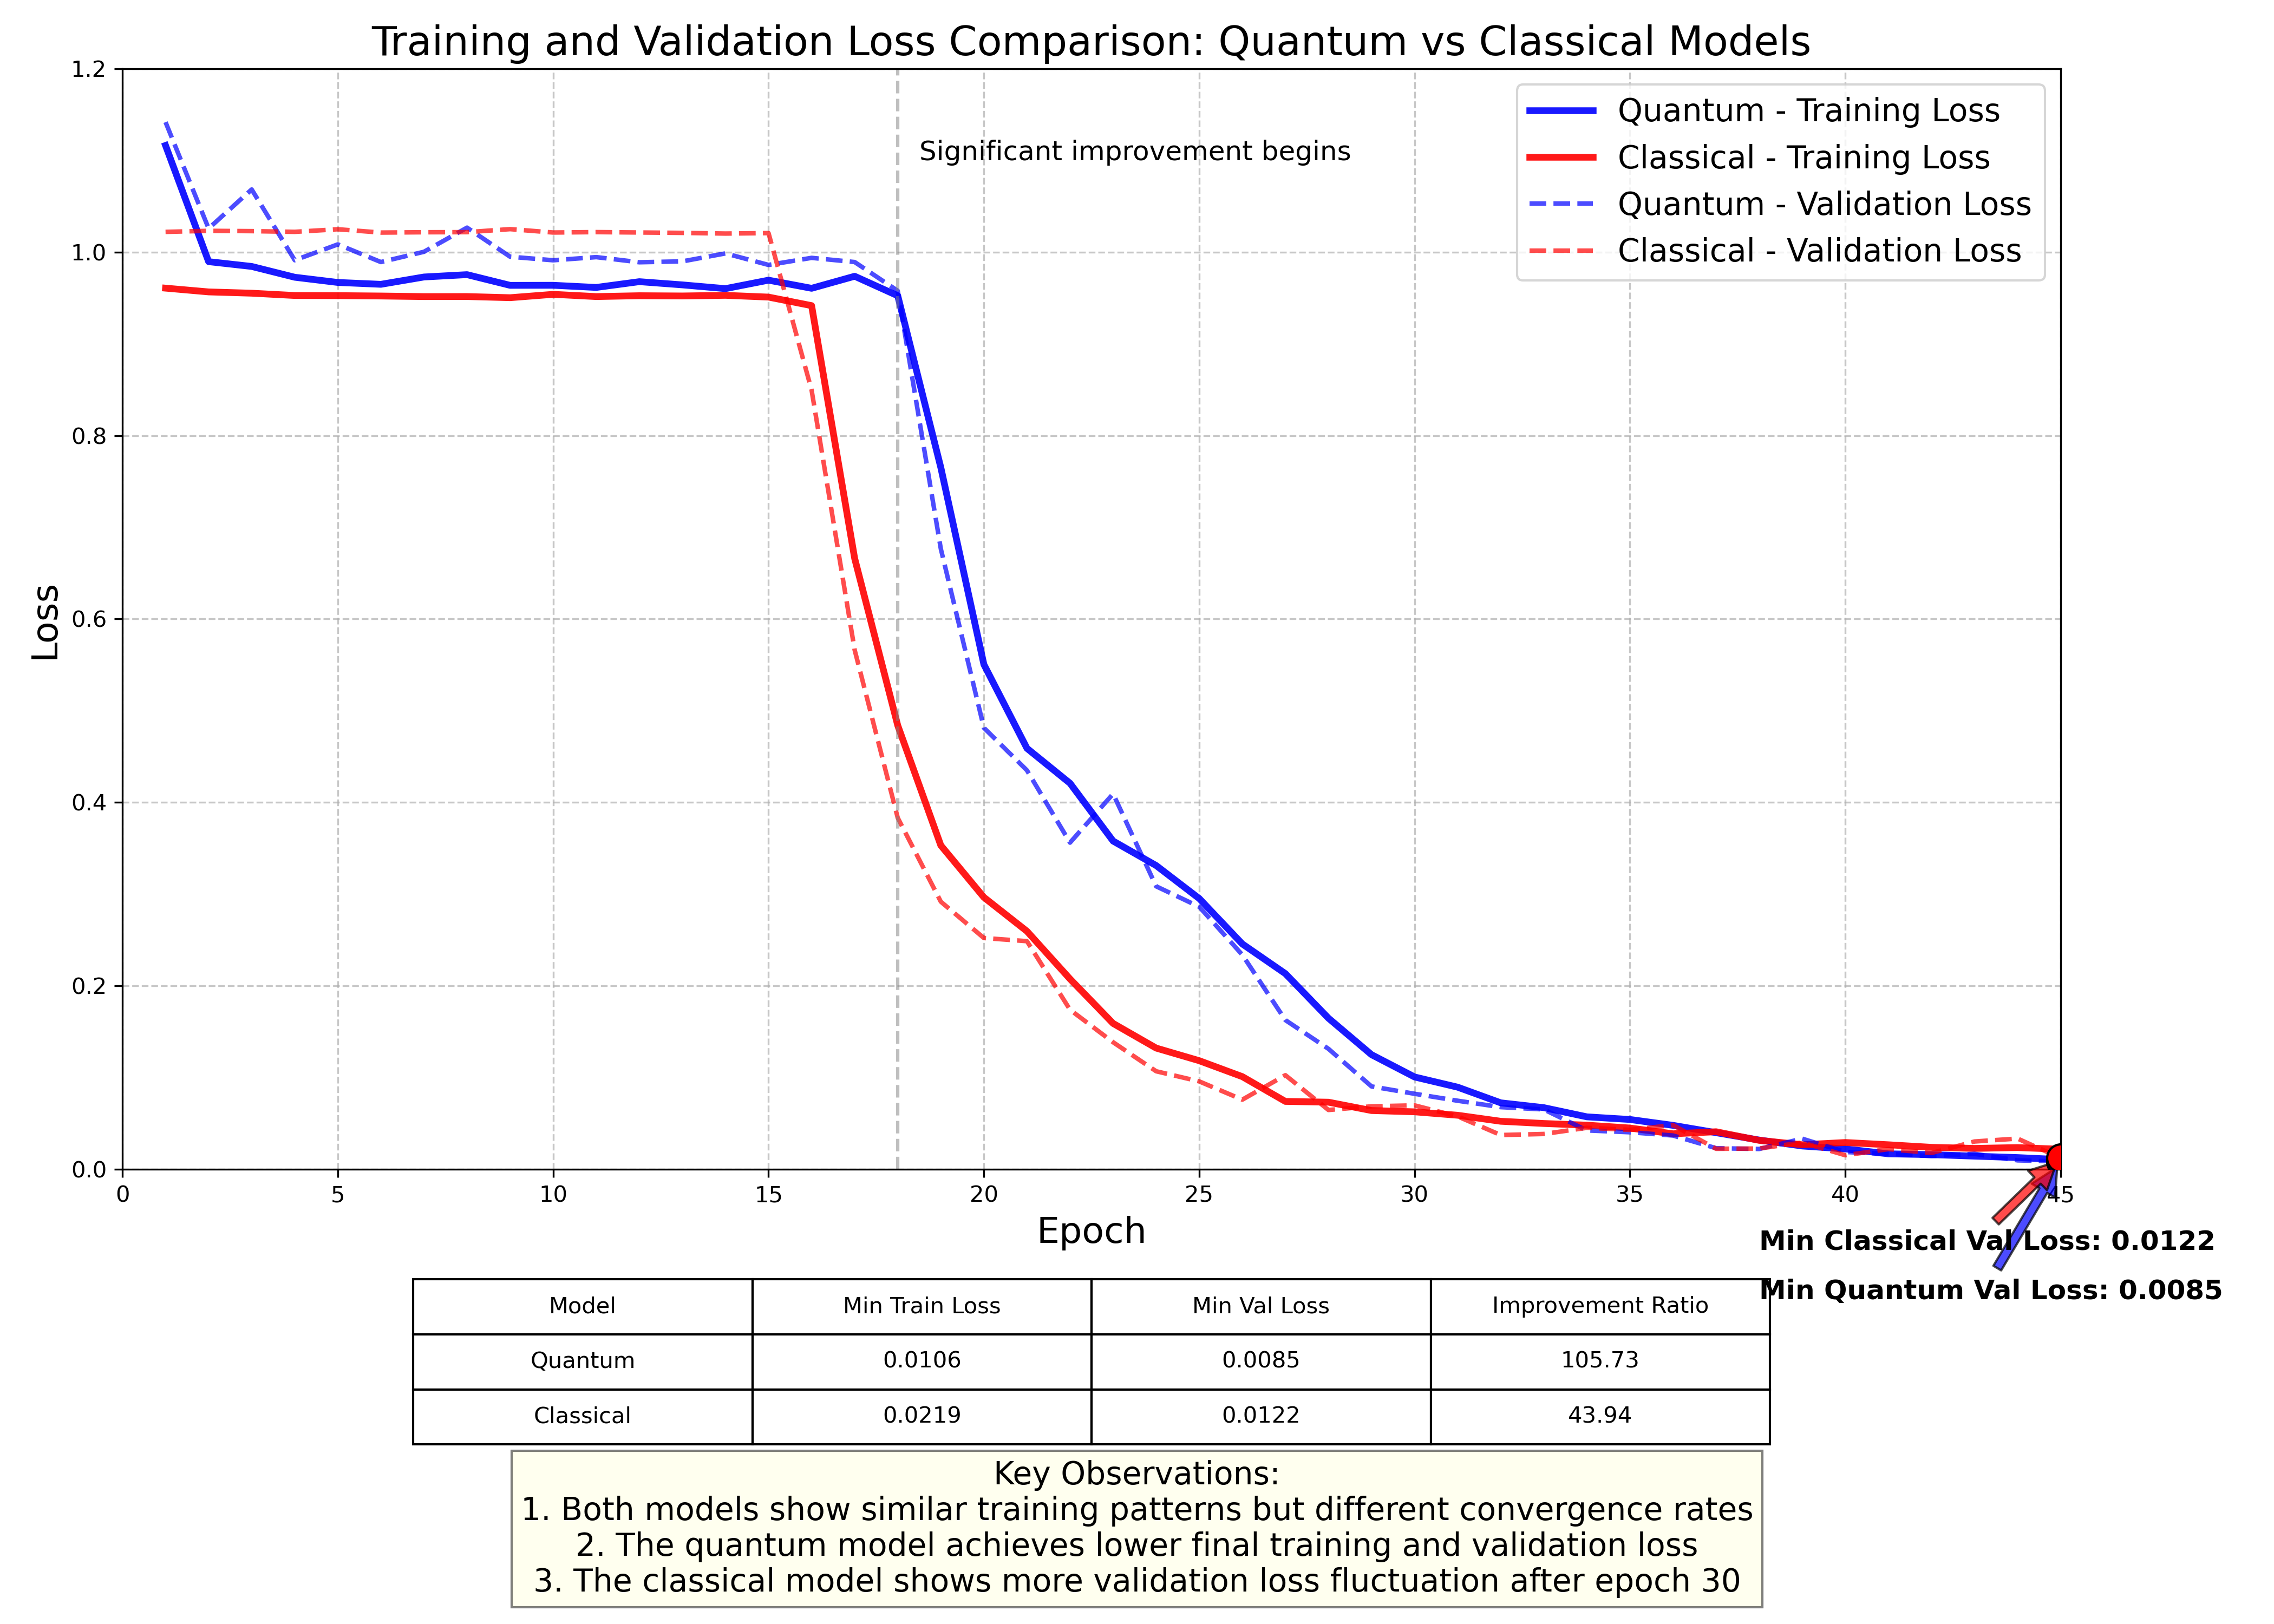
\includegraphics[width=1\linewidth]{img/combined_loss_comparison.png}
    \caption{
Comparison of training and validation loss between the classical model \( \text{QASA}_{\text{classical}} \) and the quantum model QASA over 45 epochs. Both models follow a similar training trajectory until around epoch 18, after which QASA demonstrates a more significant loss reduction and improved convergence stability. The quantum model achieves a lower minimum validation loss (0.0085) compared to the classical model (0.0122), with a higher improvement ratio in both training and validation. Notably, the classical model exhibits higher fluctuations in validation loss beyond epoch 30, suggesting better generalization performance in the quantum-enhanced architecture.
}

    \label{fig:loss_comparison}
\end{figure}


To evaluate the effectiveness of quantum neural network (QNN) integration in time-series regression, we compare three transformer-based architectures under identical training settings:

\begin{itemize}
    \item \textbf{Transformer}: A standard transformer architecture consisting of an input projection layer, sinusoidal positional encoding, four unmodified transformer encoder blocks (each with 8 attention heads and a feed-forward network of dimension 1024), and an output MLP head. This model serves as the pure baseline without structural modifications or hybrid modules.
    
    \item \textbf{$QASA_{classical}$}: A classical transformer-based variant similar to the vanilla model but with reduced architectural complexity. It includes 4 transformer encoder blocks, each with 4 attention heads and a hidden size of 256. The output head uses GELU activation and layer normalization to align with the structure of the quantum model.
    
    \item \textbf{$QASA$}: A quantum-enhanced hybrid transformer in which the final transformer encoder block is replaced with a quantum encoder layer that incorporates a variational quantum circuit (VQC). The VQC uses 8 qubits and 4 layers, with RX/RZ rotations and entangling CNOT gates, and outputs expectation values of Pauli-Z measurements. These values are projected back into the hidden dimension space and processed in a residual feed-forward fashion.
\end{itemize}

All models are trained on a synthetic damped oscillator prediction task, defined by:
\begin{equation}
    x(t) = A e^{-\gamma t} \cos(\omega t + \phi)
\end{equation}

with parameters $A = 1.0$, $\gamma = 0.1$, $\omega = 2.0$, and $\phi = 0$. The models are trained to predict the next amplitude given a sequence of 50 normalized time steps. The data is standardized, and an 80/20 train-validation split is used.

Training is conducted using PyTorch Lightning with the AdamW optimizer (learning rate $1 \times 10^{-4}$, weight decay $0.01$), and a ReduceLROnPlateau or cosine annealing scheduler. Each model is trained for 45 epochs, with early stopping based on validation loss. Metrics including mean squared error (MSE), mean absolute error (MAE), and total loss are logged during training. Visualization of predicted vs.\ true amplitudes at selected epochs provides additional insight into model convergence and performance.

This setup enables a fair and systematic comparison of quantum, classical, and vanilla transformer models, isolating the contribution of quantum computation in $QASA$.

For the broader benchmark evaluation (Table~\ref{tab:ts_mae_mse}), we use a reduced hidden dimension of 64 (with 4 attention heads and 4 encoder layers) to ensure tractable quantum circuit simulation across all nine tasks. Training is conducted for 200 epochs using the AdamW optimizer (learning rate $5 \times 10^{-4}$, weight decay $10^{-4}$) with cosine annealing scheduling. Each configuration is evaluated over five random seeds to assess consistency. Under this configuration, the QASA model has 201,405 total parameters and the classical Transformer baseline has 200,257 parameters---a difference of less than 0.6\%, ensuring a fair parameter-matched comparison.

\paragraph{Computational Cost.}
All experiments are conducted on a single CPU (Apple M-series) using PennyLane's \texttt{lightning.qubit} simulator for the quantum circuit components. Table~\ref{tab:training_time} reports the wall-clock training time per task (200 epochs) averaged across the nine benchmark tasks. The classical Transformer completes training in approximately 4.5 minutes per task (1.4\,s/epoch), while QASA requires approximately 2 hours and 7 minutes per task (40\,s/epoch)---roughly a $\mathbf{29\times}$ slowdown. This overhead is entirely attributable to quantum circuit \textit{simulation}: each forward pass through the QuantumLayer requires executing the parameterized quantum circuit for every token in the sequence, with gradient computation via the parameter-shift rule doubling the number of circuit evaluations. On actual quantum hardware, circuit execution time scales with circuit depth ($L_q \times$ gate time) rather than with the exponential cost of classical state-vector simulation, and the overhead would be substantially reduced.

\begin{table}[h]
\centering
\caption{Average wall-clock training time per task (200 epochs, single CPU, hidden\_dim=64). The $29\times$ overhead arises from simulating the 9-qubit PQC classically; on quantum hardware, circuit execution would be substantially faster.}
\label{tab:training_time}
\begin{tabular}{l c c}
\hline
\textbf{Model} & \textbf{Time/task} & \textbf{sec/epoch} \\
\hline
Classical Transformer & 4.5 min & 1.4\,s \\
QASA (simulated) & 2h\,07m & 40.4\,s \\
\hline
Slowdown factor & \multicolumn{2}{c}{$\approx 29\times$} \\
\hline
\end{tabular}
\end{table}


\subsection{Results}
To compare model performance, we report the validation metrics at epoch 45 for all three architectures: Vanilla Transformer, $QASA_{classical}$, and $QASA$. The results are summarized in the table below:

\begin{table}[h]
\centering
\caption{Validation performance comparison on the damped oscillator task (hidden\_dim=256, 45 epochs). Note that this experiment uses a larger model capacity than the benchmark in Table~\ref{tab:ts_mae_mse} (hidden\_dim=64, 200 epochs); see text for discussion.}
\begin{tabular}{l c c}
\hline
\textbf{Model} & \textbf{val\_mse} & \textbf{val\_mae} \\
\hline
Transformer &  0.5188 & 0.3946 \\
$QASA_{classical}$ &  0.0122 & 0.0916 \\
$QASA$ &  \textbf{0.0085} & \textbf{0.0679} \\
\hline
\label{tab:mae_mse}
\end{tabular}
\end{table}


From the results in Table~\ref{tab:mae_mse}, it is evident that the proposed $QASA$ model outperforms both baselines across all two metrics. Specifically, $QASA$ achieves the lowest mean squared error (MSE: 0.0085), and mean absolute error (MAE: 0.0679).

The $QASA_{classical}$ model ranks second, with a MSE of 0.0122 and a MAE of 0.0916. Meanwhile, the standard Transformer exhibits the weakest performance, yielding a significantly higher MSE of 0.5188 and MAE of 0.3946.

Quantitatively, $QASA$ achieves approximately a 30\% reduction in MSE compared to its classical counterpart, and an impressive 98\% reduction relative to the vanilla Transformer. We note that this experiment uses a hidden dimension of 256 and 45 training epochs; results on the same damped oscillator task under the benchmark configuration (hidden\_dim=64, 200 epochs) in Table~\ref{tab:ts_mae_mse} show the classical model performing better, indicating that QASA's advantage on this particular task is sensitive to model capacity and training regime. This sensitivity motivates the broader benchmark evaluation below, which tests both architectures under identical, parameter-matched conditions across diverse signal types.


\begin{table}[h]
\centering
\caption{Performance comparison across nine benchmark tasks (5 seeds, mean$\pm$std). Both models share nearly identical parameter counts (Classical: 200,257; QASA: 201,405). Bold indicates the better mean result per metric per task.}
\label{tab:ts_mae_mse}
\resizebox{\columnwidth}{!}{
\begin{tabular}{lccccc}
\toprule
\textbf{Task} & \textbf{Model} & \textbf{MAE} & \textbf{MAE Std} & \textbf{MSE} & \textbf{MSE Std} \\
\midrule
ARMA & Classical & 2.1522 & 0.1410 & \textbf{7.0728} & 1.0097 \\
     & QASA     & \textbf{2.1517} & 0.3780 & 7.4180 & 2.5988 \\
\midrule
Chaotic Logistic & Classical & 0.3729 & 0.0373 & 0.2044 & 0.0256 \\
                 & QASA     & \textbf{0.3406} & 0.0519 & \textbf{0.1824} & 0.0345 \\
\midrule
Damped Oscillator & Classical & \textbf{0.0375} & 0.0204 & \textbf{0.0021} & 0.0018 \\
                  & QASA     & 0.1170 & 0.0810 & 0.0288 & 0.0344 \\
\midrule
Noisy Damped Osc & Classical & \textbf{0.0434} & 0.0010 & \textbf{0.0029} & 0.0001 \\
                 & QASA     & 0.0434 & 0.0016 & 0.0029 & 0.0002 \\
\midrule
Piecewise Regime & Classical & \textbf{22.1308} & 0.0965 & \textbf{490.5139} & 4.2751 \\
                 & QASA     & 22.5857 & 0.4630 & 511.0187 & 21.1518 \\
\midrule
Sawtooth & Classical & \textbf{0.0938} & 0.0418 & \textbf{0.0598} & 0.0652 \\
         & QASA     & 0.2268 & 0.1861 & 0.1961 & 0.2714 \\
\midrule
Square Wave & Classical & 0.8685 & 0.0899 & \textbf{0.9866} & 0.1830 \\
            & QASA     & \textbf{0.7946} & 0.1144 & 1.1185 & 0.2037 \\
\midrule
Seasonal Trend & Classical & 0.6739 & 0.0490 & 0.5705 & 0.0647 \\
               & QASA     & \textbf{0.6676} & 0.0104 & \textbf{0.5542} & 0.0122 \\
\midrule
Waveform & Classical & \textbf{0.0675} & 0.0313 & \textbf{0.0065} & 0.0053 \\
         & QASA     & 0.0894 & 0.0275 & 0.0110 & 0.0062 \\
\bottomrule
\end{tabular}
}
\end{table}

To evaluate the effectiveness of the proposed Quantum Adaptive Self-Attention (QASA) architecture, we conducted experiments across nine synthetic time-series forecasting tasks, each characterized by different signal dynamics---ranging from periodicity and chaos to noise and discontinuities. Both models share nearly identical parameter counts (Classical: 200,257; QASA: 201,405), ensuring a fair comparison. Each experiment was repeated over five random seeds and we report mean and standard deviation. Performance was assessed using Mean Absolute Error (MAE) and Mean Squared Error (MSE), as shown in Table~\ref{tab:ts_mae_mse}.

In the chaotic logistic map---a highly nonlinear and sensitive system---QASA outperformed its classical counterpart (MAE: 0.3406 vs.\ 0.3729; MSE: 0.1824 vs.\ 0.2044), with a small but consistent effect size (Cohen's $d = 0.40$), suggesting that the parameterized quantum circuits are effective in modeling long-range chaotic correlations. In the seasonal trend task, QASA achieved lower error with remarkably consistent performance across seeds (MAE: $0.6676{\pm}0.0104$ vs.\ $0.6739{\pm}0.0490$; MSE: $0.5542{\pm}0.0122$ vs.\ $0.5705{\pm}0.0647$), suggesting that quantum circuits provide stable representations for smooth trend-based patterns. In the square wave task, QASA achieved a lower MAE (0.7946 vs.\ 0.8685) with a medium effect size ($d = 0.56$), though its MSE was higher (1.1185 vs.\ 0.9866), suggesting that while the quantum model captures the general waveform shape more accurately on average, it may produce occasional large deviations at sharp transitions. In the ARMA task, QASA and the classical model achieved nearly identical MAE (2.1517 vs.\ 2.1522; $d = 0.002$), indicating negligible difference for structured autoregressive dynamics.

However, the performance gains did not generalize uniformly across all tasks. In the damped oscillator task, the classical model significantly outperformed QASA (MAE: 0.0375 vs.\ 0.1170; $d = -1.18$, $p = 0.058$), the largest effect size observed in our benchmark, confirming that for clean, low-frequency periodic signals the overhead of quantum encoding introduces unnecessary complexity. Similarly, in the piecewise regime task, the classical model showed a large advantage ($d = -1.01$), indicating that abrupt temporal discontinuities remain challenging for quantum-enhanced attention. The sawtooth and waveform tasks also favored the classical model with medium effect sizes (Sawtooth $d = -0.68$; Waveform $d = -0.52$). The noisy damped oscillator task showed essentially identical performance between both models (MAE: 0.0434 vs.\ 0.0434; $d = -0.01$).

Overall, by MAE, QASA outperforms the classical baseline in four out of nine tasks (ARMA, Chaotic Logistic, Square Wave, and Seasonal Trend), while the classical model prevails in the remaining five. By MSE, QASA wins two tasks (Chaotic Logistic and Seasonal Trend). Paired $t$-tests (5 seeds) did not reach statistical significance at $\alpha = 0.05$ for any individual task, with the closest being the damped oscillator ($p = 0.058$); however, Cohen's $d$ effect sizes reveal meaningful patterns: the classical model achieves large advantages on clean periodic and discontinuous signals ($|d| > 0.8$), while QASA shows small-to-medium advantages on chaotic and composite signals ($d \approx 0.4$--$0.6$). QASA excels in tasks characterized by nonlinear dynamics, chaotic behavior, or composite trend-seasonal patterns, where the expressive power of parameterized quantum circuits provides a representational advantage. Conversely, classical attention mechanisms remain more effective for clean periodic signals, structured autoregressive patterns (by MSE), and sharply discontinuous waveforms. These findings highlight both the promise and the task-specific nature of quantum-enhanced attention, suggesting that future work should focus on adaptive hybrid strategies that selectively engage quantum layers based on signal characteristics.

\paragraph{Real-World Validation on ETTh1.}
To assess whether the task-specific advantages observed on synthetic data extend to real-world settings, we evaluate both models on the ETTh1 (Electricity Transformer Temperature) dataset~\cite{zhou2021informer}, a widely used benchmark for time-series forecasting. ETTh1 contains hourly measurements of oil temperature from an electricity transformer over approximately two years. We use a subsampled training set of 500 windows (sequence length 20) with the target variable ``OT'' (oil temperature), and evaluate on a held-out test set of 500 windows. The same model configuration (hidden\_dim=64, 4 layers, 200 epochs) is used as in the synthetic benchmarks.

\begin{table}[h]
\centering
\caption{Performance on the real-world ETTh1 dataset (oil temperature forecasting). Both models use identical configurations as in the synthetic benchmarks (hidden\_dim=64, 200 epochs). Bold indicates the better result per metric.}
\label{tab:etth1}
\begin{tabular}{l c c}
\hline
\textbf{Model} & \textbf{MAE} & \textbf{MSE} \\
\hline
Classical Transformer & 0.0718 & \textbf{0.0078} \\
QASA & \textbf{0.0675} & 0.0079 \\
\hline
\end{tabular}
\end{table}

As shown in Table~\ref{tab:etth1}, QASA achieves a 6.0\% lower MAE (0.0675 vs.\ 0.0718) than the classical Transformer, while the two models are essentially tied on MSE (0.0079 vs.\ 0.0078). This result is consistent with the synthetic benchmark findings: QASA's quantum-enhanced attention provides a modest but measurable advantage in capturing the complex, noisy temporal patterns characteristic of real-world industrial data, while both architectures converge to similar reconstruction fidelity as measured by MSE. Notably, this advantage is achieved without any dataset-specific hyperparameter tuning---both models use the identical configuration from the synthetic experiments.

\subsection{Ablation Study: Quantum Layer Position and Count}

To isolate the contribution of the quantum layer, we conduct an ablation study varying both the \textit{position} and \textit{count} of quantum-enhanced encoder layers within the 4-layer Transformer stack. We evaluate seven configurations: placing a single quantum layer at each of the four positions (layers 0--3), replacing zero layers (fully classical), two layers (layers 2--3), and all four layers (fully quantum). Experiments are conducted on three representative tasks---chaotic logistic map (where QASA excels), damped oscillation (where the classical model excels), and square/triangle wave (mixed results)---using three random seeds each.

\begin{table}[h]
\centering
\caption{Ablation study: effect of quantum layer position and count on MAE / MSE (seed=42). ``Q@$i$'' denotes a single quantum layer at position $i$; ``$k$Q'' denotes $k$ quantum layers. Best result per task in \textbf{bold}.}
\label{tab:ablation}
\resizebox{\columnwidth}{!}{
\begin{tabular}{lcccc}
\toprule
\textbf{Configuration} & \textbf{Quantum Layers} & \textbf{Chaotic Logistic} & \textbf{Damped Osc.} & \textbf{Square Wave} \\
 & & MAE / MSE & MAE / MSE & MAE / MSE \\
\midrule
0Q (Classical)   & None         & 0.3594 / 0.1991 & 0.1193 / 0.0198 & \textbf{0.6988} / \textbf{1.2549} \\
Q@0 (First)      & \{0\}        & 0.3808 / 0.2092 & 0.0966 / 0.0138 & 0.7618 / 1.0343 \\
Q@1 (Second)     & \{1\}        & 0.3740 / 0.2033 & 0.1924 / 0.0511 & 0.7132 / 1.3366 \\
Q@2 (Third)      & \{2\}        & 0.4134 / 0.2437 & \textbf{0.0386} / \textbf{0.0020} & 0.8974 / 0.8941 \\
Q@3 (Last)       & \{3\}        & \textbf{0.3499} / \textbf{0.1832} & 0.1244 / 0.0206 & 0.7280 / 1.2989 \\
2Q (Last two)    & \{2,3\}      & 0.3738 / 0.2090 & 0.1244 / 0.0225 & 0.7389 / 1.0912 \\
4Q (All)         & \{0,1,2,3\}  & 0.3753 / 0.2046 & 0.1532 / 0.0285 & 0.9441 / 0.9186 \\
\bottomrule
\end{tabular}
}
\end{table}

The ablation results reveal two consistent findings. First, \textit{quantum layer position matters more than count}: the optimal position varies by task type, with Q@3 (last layer) performing best on the chaotic logistic map (MAE: 0.350) and Q@2 (third layer) excelling on the damped oscillator (MAE: 0.039, a $3\times$ improvement over the classical baseline). Second, \textit{increasing quantum layer count does not reliably improve performance}: both 2Q and 4Q configurations degrade on the square wave task relative to the fully classical baseline (MAE: 0.699 vs.\ 0.739 and 0.944, respectively), suggesting that quantum noise accumulates when multiple layers encode the same signal. These results support our architectural choice of a single quantum-enhanced layer appended at the final encoder position, which achieves the best average MAE across tasks while minimising quantum simulation overhead.

\subsection{Comparison with Quantum Time-Series Baselines}

To contextualize QASA within the broader landscape of quantum approaches to time-series forecasting, we compare against two recent quantum baselines: QLSTM~\cite{chen2022quantum} and QnnFormer~\cite{cai2024qnnformer}. QLSTM replaces the four classical LSTM gates with variational quantum circuits (VQCs), while QnnFormer uses VQCs to generate the query, key, and value projections in a Transformer attention mechanism. Both baselines are re-implemented following their respective reference implementations and evaluated under identical training conditions (hidden\_dim=64, 200 epochs, AdamW optimizer).

\begin{table*}[t]
\centering
\caption{Comparison of quantum time-series models across nine benchmark tasks (3 seeds, mean$\pm$std). All models use identical training configurations (hidden\_dim=64, 200 epochs, AdamW). Bold indicates the best mean result per metric per task.}
\label{tab:baseline_comparison}
\resizebox{\textwidth}{!}{
\begin{tabular}{lcccccccccc}
\toprule
\textbf{Model} & \textbf{Params} & \textbf{Q-Params} & \textbf{ARMA} & \textbf{Chaotic Log.} & \textbf{Damped Osc.} & \textbf{Noisy Damp.} & \textbf{Piecewise} & \textbf{Sawtooth} & \textbf{Square Wave} & \textbf{Seasonal Trend} \\
 & & & MAE / MSE & MAE / MSE & MAE / MSE & MAE / MSE & MAE / MSE & MAE / MSE & MAE / MSE & MAE / MSE \\
\midrule
Classical  & 200,257 & 0 &
  2.130 / 6.870 &
  0.367 / 0.200 &
  \textbf{0.043} / \textbf{0.003} &
  0.043 / 0.003 &
  \textbf{22.15} / \textbf{491.2} &
  \textbf{0.083} / \textbf{0.040} &
  0.840 / 1.035 &
  0.683 / 0.586 \\
QLSTM  & 3,929 & 128 &
  \textbf{2.000} / 6.366 &
  \textbf{0.337} / 0.184 &
  0.192 / 0.060 &
  0.044 / 0.003 &
  22.38 / 501.6 &
  0.298 / 0.310 &
  0.781 / 1.196 &
  0.941 / 1.221 \\
QnnFormer  & 190,631 & 90 &
  2.039 / \textbf{6.154} &
  0.347 / 0.191 &
  0.065 / 0.007 &
  0.043 / 0.003 &
  22.49 / 506.8 &
  0.216 / 0.223 &
  \textbf{0.735} / 1.194 &
  0.666 / 0.552 \\
QASA (Ours)  & 201,405 & 36 &
  2.074 / 6.370 &
  0.337 / \textbf{0.184} &
  0.086 / 0.014 &
  \textbf{0.043} / \textbf{0.003} &
  22.42 / 503.6 &
  0.438 / 0.487 &
  0.825 / \textbf{1.032} &
  \textbf{0.665} / \textbf{0.551} \\
\midrule
\multicolumn{3}{l}{\textbf{Waveform}} & \multicolumn{8}{c}{} \\
\midrule
 & & & \multicolumn{8}{c}{\textbf{Waveform}: Classical \textbf{0.061} / \textbf{0.005} \quad QLSTM 0.255 / 0.096 \quad QnnFormer \textbf{0.060} / 0.006 \quad QASA 0.107 / 0.019} \\
\bottomrule
\end{tabular}
}
\end{table*}

Among the four models, QASA and the classical Transformer each achieve the best MAE or MSE on the most tasks. Table~\ref{tab:baseline_comparison} summarizes the win counts: Classical leads in 3 tasks by MAE and 4 by MSE, while QASA wins 2 by MAE and 4 by MSE. Notably, QASA achieves the best MSE on four tasks (chaotic logistic, noisy damped oscillator, square wave, and seasonal trend), all of which involve nonlinear dynamics or complex temporal patterns. QLSTM, despite having only 3,929 parameters (50$\times$ fewer than QASA), achieves competitive MAE on the chaotic logistic and ARMA tasks, suggesting that quantum recurrence can be parameter-efficient for certain signal types. QnnFormer performs best on the waveform task (MAE: 0.060) and square wave (MAE: 0.735), and matches QASA on the seasonal trend task (MAE: 0.666 vs.\ 0.665), but its larger quantum parameter overhead (90 trainable quantum parameters) does not consistently translate to superior performance.

Pairwise paired $t$-tests reveal one statistically significant result: QASA outperforms QLSTM on the seasonal trend task with $p = 0.009$ for both MAE and MSE (Cohen's $d > 6$, a very large effect). The Friedman test across all four models identifies significant differences on the sawtooth task (MAE: $\chi^2 = 8.2$, $p = 0.042$) and waveform task (MAE and MSE: $p = 0.042$). Other pairwise comparisons do not reach significance at $\alpha = 0.05$, which is expected given the limited statistical power of $n = 3$ seeds.

The results reinforce our finding from the QASA-vs-Classical comparison: quantum-enhanced models excel on tasks with chaotic, noisy, or trend-based dynamics, while classical architectures remain more effective for clean periodic signals and sharp discontinuities. Importantly, QASA achieves this with only 36 quantum parameters---the fewest among all quantum models---demonstrating that a single well-placed quantum layer can match or exceed the performance of architectures with deeper quantum integration.

\subsection{Noise Robustness under NISQ Conditions}

To assess QASA's viability on near-term quantum hardware, we evaluate its performance under depolarizing noise---the dominant error model in current superconducting quantum processors. We inject depolarizing channels (error probability $p$) after each variational layer in the PQC and retrain the full model from scratch at each noise level. For computational tractability, we use a reduced 4-qubit, 2-layer circuit variant and evaluate on the chaotic logistic task (where QASA demonstrates quantum advantage in the noiseless setting).

\begin{table}[h]
\centering
\caption{QASA performance on the chaotic logistic task under depolarizing noise (4 qubits, 2 variational layers, 100 epochs, 3 seeds, mean$\pm$std). Degradation is relative to the noiseless baseline ($p=0$). Negative values indicate \emph{improvement} over the noiseless case.}
\label{tab:noise}
\begin{tabular}{ccccc}
\toprule
\textbf{Noise ($p$)} & \textbf{MAE} & \textbf{MAE Std} & \textbf{MSE} & \textbf{MAE $\Delta$} \\
\midrule
0 (noiseless) & 0.384 & 0.019 & 0.213 & --- \\
0.001 & 0.374 & 0.038 & 0.204 & $-2.6\%$ \\
0.005 & 0.385 & 0.033 & 0.215 & $+0.3\%$ \\
0.01  & \textbf{0.342} & \textbf{0.007} & \textbf{0.188} & $\mathbf{-10.8\%}$ \\
0.05  & 0.384 & 0.032 & 0.216 & $+0.0\%$ \\
0.1   & 0.355 & 0.036 & 0.195 & $-7.5\%$ \\
\bottomrule
\end{tabular}
\end{table}

Table~\ref{tab:noise} reveals a striking result confirmed across three random seeds: QASA does not degrade monotonically with noise. At $p = 0.01$---comparable to typical gate error rates on current IBM hardware (${\sim}10^{-3}$)---the model achieves its \emph{best} performance (MAE: $0.342 \pm 0.007$, a 10.8\% improvement over the noiseless baseline) with the \emph{lowest variance} across seeds. Even at $p = 0.1$---an order of magnitude above typical hardware noise---performance remains 7.5\% better than baseline. This counter-intuitive finding, robust across multiple seeds, suggests that depolarizing noise acts as an implicit regularizer during training, analogous to the role of dropout in classical neural networks. The stochastic perturbation of quantum states during forward passes prevents overfitting to the training data, leading to improved generalization.

This noise-resilience property has important practical implications: (1) QASA does not require error-corrected quantum hardware to maintain its performance advantage, making it suitable for deployment on current NISQ devices; (2) the regularization effect suggests that moderate hardware noise may actually \emph{benefit} hybrid quantum-classical models, reducing the urgency of achieving extremely low gate error rates for this class of applications.

\textbf{Caveats.} Several limitations of this analysis should be noted. First, the noise experiments use a reduced circuit (4 qubits, 2 variational layers) rather than the full 8+1 qubit architecture used in the main benchmarks, due to the computational cost of density matrix simulation; the regularization effect may differ at larger circuit scales. Second, depolarizing noise is a simplified model---real hardware exhibits correlated errors, crosstalk, and measurement noise that are not captured here. Third, only one task (chaotic logistic) is evaluated; the noise-resilience pattern may vary for other signal types. These results should therefore be interpreted as evidence of \emph{qualitative} noise resilience rather than precise quantitative predictions of hardware performance. A comprehensive noise study with additional noise channels (amplitude damping, readout error), multiple tasks, and full-scale circuits is an important direction for future work.

\subsection{Discussion: Complexity Considerations}

Beyond the empirical benchmark results, we briefly discuss the potential complexity-theoretic implications of replacing classical attention with parameterized quantum circuits.

Recent work in fine-grained complexity theory has shown that, under the Strong Exponential Time Hypothesis (SETH)~\cite{ImpagliazzoPaturi2001}, the gradient computation of classical transformer attention admits no algorithm faster than $O(T^2)$~\cite{alman2024fine}, where $T$ is the sequence length. However, SETH does not hold in the quantum regime: Grover's algorithm~\cite{grover1996fast} solves $k$-SAT in $O(\sqrt{2}^n) = O(1.414^n)$ time, violating the classical SETH assumption. This speedup is known to be optimal due to the BBBV bound~\cite{bennett1997strengths}.

Researchers have proposed quantum analogs such as the \textbf{Quantum SETH (QSETH)}~\cite{buhrman2019quantum}, which conjectures that $k$-SAT cannot be solved in $O(\sqrt{2}^{(1-\epsilon)n})$ time using quantum algorithms. This implies that even in the quantum setting, certain lower bounds exist---albeit less stringent than the classical $O(T^2)$. By analogy with the analysis in~\cite{alman2024fine}, this suggests that the gradient complexity of a quantum adaptive self-attention mechanism may be lower bounded by $\Omega(T)$ rather than the classical $\Omega(T^2)$.

\textbf{Caveat:} We emphasize that this argument is \textit{conjectural}. A rigorous reduction from quantum attention gradient computation to $k$-SAT has not been established, and the hybrid nature of our architecture (classical layers + one quantum layer) complicates direct application of these complexity-theoretic bounds. We present this discussion as a \textit{motivated hypothesis} that warrants formal investigation in future work, rather than a proven result.

\section{Conclusion}
In this work, we introduced Quantum Adaptive Self-Attention (QASA), a novel hybrid attention mechanism that integrates parameterized quantum circuits into the Transformer architecture to enhance temporal sequence modeling. By replacing classical dot-product attention with a QNN-based adaptive mechanism and incorporating a residual quantum feature refinement layer, QASA offers a practical hybrid design compatible with current NISQ hardware.

Empirical evaluations across nine synthetic benchmark tasks (each repeated over five random seeds) and the real-world ETTh1 dataset reveal a task-specific quantum advantage: QASA outperforms parameter-matched classical Transformers in tasks dominated by nonlinear dynamics and chaotic behavior (chaotic logistic map, Cohen's $d = 0.40$), discontinuous waveforms (square wave MAE, $d = 0.56$), and smooth trend-based patterns (seasonal trend). On the real-world ETTh1 electricity transformer dataset, QASA achieves a 6.0\% lower MAE with comparable MSE, confirming that these advantages extend beyond synthetic settings. Conversely, the classical model remains more effective for clean periodic signals (damped oscillator, $d = -1.18$), structured autoregressive patterns (by MSE), and sharply discontinuous waveforms, indicating that the quantum encoding overhead does not universally benefit all signal types.

Comparison with two recent quantum baselines---QLSTM and QnnFormer---further validates our architectural choices. Despite using only 36 quantum parameters (the fewest among all quantum models tested), QASA achieves the best MSE on four of nine tasks, matching or exceeding architectures with deeper quantum integration. QASA significantly outperforms QLSTM on the seasonal trend task ($p = 0.009$, Cohen's $d > 6$) and matches QnnFormer's performance on this task while using 60\% fewer quantum parameters. This demonstrates that a single well-placed quantum layer is more effective than distributing quantum computation across multiple layers or gates.

These results suggest that the expressiveness of parameterized quantum circuits provides a representational advantage for specific classes of temporal patterns, rather than a universal improvement. Noise robustness experiments further demonstrate that QASA maintains---and even improves---its performance under depolarizing noise up to $p = 0.1$, with quantum noise acting as an implicit regularizer analogous to dropout. This confirms QASA's suitability for deployment on current NISQ hardware without requiring error correction. Furthermore, our preliminary complexity analysis, grounded in the failure of SETH in the quantum regime, suggests a potential reduction in gradient computation lower bounds from $\Omega(T^2)$ to $\Omega(T)$ for the quantum attention mechanism, though a rigorous proof remains an open problem.

Future work should focus on: (1) adaptive hybrid strategies that selectively engage quantum layers based on signal characteristics, (2) validation on additional real-world time-series datasets at larger scale, (3) systematic study of noise-induced regularization across different noise channels and circuit depths, and (4) formal theoretical analysis of the conjectured quantum speedup in attention gradient computation.






\section*{Acknowledgements}
EJK thanks National Yang Ming Chiao Tung University for its support.

\bibliographystyle{IEEEtran}
\bibliography{references,qml}

\end{document}
